\documentclass{article}
\usepackage[utf8]{inputenc}
\usepackage{url}
\usepackage[margin=1in]{geometry}
\usepackage{parskip}
\usepackage{natbib}
\usepackage{graphicx}
\usepackage{booktabs}
\usepackage[binary-units=true]{siunitx}
\usepackage{listings}
\usepackage{scrextend}
\usepackage{caption}
\usepackage{subcaption}
\usepackage{placeins}




\title{Big Data Random Forests in R}
\author{Andrew Nisbet }
\date{April 2016}



\begin{document}

\maketitle

\section{Introduction}
This project investigates using R to perform random forest classification on a large dataset of flight information. Several methods are applied to various sample sizes. The aim is to better understand the limitations of R, and how  to handle random forest classification for a given dataset size.

In particular, the packages \texttt{randomForest} \cite{rf} and \texttt{bigrf} \cite{bigrf} are compared.

The performance aspects evaluated are run time, RAM usage, and whether the program crashes. Model accuracy is also considered, but it is not the focus of the project.


\section{Working With Big Data}

There is a large performance difference between file storage (hard drive) and working memory (RAM) in a computer. Here are the approximate performance benchmarks for my laptop:

\begin{table}[h!]
\centering
\begin{tabular}{ l c c }
  \toprule
  & Hard Drive & RAM\\
  \midrule
  Free Capacity & \SI{200}{\giga\byte} & \SI{4}{\giga\byte}\\
  Transfer Rate & \SI{50}{\mega\byte\per\second} & \SI{5000}{\mega\byte\per\second} \\
  Access Delay & \SI{10000000}{\nano\second} & \SI{10}{\nano\second}  \\
  \bottomrule
\end{tabular}
\end{table}

RAM is many orders of magnitude faster than hard drives, and for this reason most statistical software  stores all variables and intermediate computations in RAM. However, as datasets get larger and computations get more complex, this information may no longer fit, causing the program to crash.

There are many ways to reduce RAM usage, some of which are seen in this project:
\begin{itemize}
    \item[] \textbf{Sampling} Dataset size suffers from diminishing returns: At a certain size there is negligible accuracy gained by increasing the number of observations $n$. This is analysed by comparing the classification error for dataset subsets of different sizes.
    \item[] \textbf{Streaming} Some packages are able to stream large files: reading and processing a single line at a time. This works for methods that only apply to each line (e.g. replacing \texttt{NA}s rather than computing a column mean) and for text-based files (e.g. \texttt{.csv} files rather than databases). Streaming is also used to create training samples of different sizes.
    \item[] \textbf{Ensemble methods} Some statistical algorithms can be trained on subsets of the data, then the resulting models can be averaged. Random forests are perfectly suited for this optimisation: A random forest is a combination of individual trees, each trained on subsets of the data features. 
    % Forests can also be trained on different subsets of the observations, this technique will also be examined.
    \item[] \textbf{Lazy loading} Because random forest computations are only working on a subset of the data at a time, the extra data can be stored on disk then loaded in to RAM just before it is needed. This technique is what separates the \texttt{bigrf} package from the standard \texttt{randomForest} package, and should allow the former to better cope with large datasets.
    
\end{itemize}

These techniques will be used in a variety of ways in this project. But first, we need some data to work with.

\section{The Dataset}
\subsection{Sources}
The dataset chosen for this project consists of details for all domestic flights in the United States between 1987 and 2008 \cite{asa}. Cleaned data is provided by the American Statistics Association as part of a data visualisation competition. The dataset contains 28 features for 120 million flights, and is \SI{12}{\giga\byte} in size.

Random forests models were used to predict whether a flight would be delayed.

On average 27\% of flights in the data are delayed, so a classification error less than this represents an improvement on guessing. Because the focus of the project is to experiment with R rather than to produce the best possible model, we will ignore more accurate measures of error for skewed samples such as precision and recall. All errors reported are run on a separate validation sample.

An initial test on a small subset of the data resulted in classifications no better than guessing. But this is perhaps not so surprising: If an airline recognised that a certain flight was consistently delayed it would adjust the scheduled flight time. Airlines have been doing big data for a long time.

In order to predict delay better than the airlines, we need data not available at the time the schedule is set - namely weather data. The National Oceanic and Atmospheric Administration (NOAA) provides weather reading data for the 14,000 stations they maintain across the United States, in hourly resolution for the past 100 years \cite{noaa}.

Finally, the data needed to be processed to link the flight and weather datasets.

\subsection{Processing}

The data was processed as follows
\begin{itemize}
    \item Flight data was downloaded from the American Statistics Association.
    \item The flight departure and arrival times are recorded in the local timezone, while the weather data uses UTC time. The local times were converted by finding the timezone of each airport \cite{tzmap}, and then the time offset for each timezone \cite{wikitz}.
    \item In the flight data, airports are referenced by their FAA callsign (e.g. LAX), while the weather data uses its own weather station number. The NOAA provides a list of all weather station numbers \cite{wban}.
    \item Weather data was downloaded from NOAA for the airport monitoring stations, and combined with the fight data using the time and station number.
\end{itemize}

The downloading and processing was performed by a combination of R, Python, and Bash code. The weather data for the airport weather stations is split into 5000 files, which needed to be downloaded in parallel to finish in a reasonable time.

For processing, much use was made of Python's \texttt{map()} and R's \texttt{apply()} functions, which stream through a dataset and apply a function to each row at a time, allowing you to perform complex transforms of the data without using a significant amount of memory. In some cases, this technique was better (perhaps slower, but didn't crash) than using builtin vectorised functions.

The combined flight and weather data was \SI{15}{\giga\byte} in size.

\subsection{Feature Selection}
Features were chosen to imitate the information that would be known at boarding, excluding information like taxi times. Semi-duplicate features such as air time and flight distance were deduplicated.

From the flight data, the following features were kept:
\begin{itemize}
    \item Year
    \item Month
    \item Day of the week
    \item Hour of the day (at origin and destination)
    \item Airline
    \item Flight duration
    \item Destination airport code
    \item Whether boarding was delayed
\end{itemize}
All features except for flight duration were converted to categorical features.

From the weather data, the following features for both the origin and destination airports were used:
\begin{itemize}
    \item Temperature
    \item Air pressure
    \item Wind speed
    \item Amount of cloud cover (categorical)
    \item Precipitation
\end{itemize}

The $y$ feature for prediction was whether the flight landed more than 15 minutes later than scheduled, a standard measure of delay. There was no missing data for this feature.

Finally, the data was restricted to those flights departing from Chicago O'Hare Airport, chosen because it is one of the largest airports with one of the highest delay rates.

Approximately 5\% of weather data points were missing: these rows were dropped from the dataset, as there was no correlation between missing weather and flight delay. For the remaining observations, about 10\% had data missing for a single weather feature: Missing values were filled in with the median or mode of the column, for continuous and categorical features respectively. 

The final dataset was \SI{500}{\mega\byte} in size, with 5 million rows and 19 features. Although small enough to be processed by R with little effort, this is large enough to pose RAM challenges to the random forest packages.


\subsection{Sampling}
The data was split into a validation set of 10000 observations, and the remainder into a training set. Both random forest packages perform their own test/train splitting.

Subsets of the training data were made with different sizes. To investigate working with large data, several methods for creating subsets from the \SI{500}{\mega\byte} dataset were investigated.

A naive approach in R using the builtin \texttt{read.csv} caused the program to crash from lack of RAM:
\begin{lstlisting}[frame=single, basicstyle=\footnotesize\ttfamily]
df <- read.csv(from.filename, header=TRUE)
write.csv(file=to.filename, x=df[sample(nrow(df), n.samples), ], row.names=FALSE)
\end{lstlisting}

Performance can be improved by reading the first few lines of the file and using those to determine the column classes. This prevents R from processing the entirety of each column to compute the classes. Passing the number of lines of the file (found using the linux command line tool \texttt{wc -l}) allows R to allocate RAM for the file in advance:
\begin{lstlisting}[frame=single, basicstyle=\footnotesize\ttfamily]
df.head <- read.table(from.filename, header=TRUE, nrows=5)
classes <- sapply(df.head, class)
df <- read.table(from.filename, header=TRUE, nrows=7009729)
write.csv(file=to.filename, x=df[sample(nrow(df), n.samples),
\end{lstlisting}
The sampling completed in \SI{260}{\second}.

However, when working with large files in R, it is usually better to use the \texttt{fread} function from the \texttt{data.table} library. It performs all of the above performance optimisations and completed significantly faster, in \SI{16}{\second}:
\begin{lstlisting}[frame=single, basicstyle=\footnotesize\ttfamily]
library(data.table)
df <- fread(from.filename, header=TRUE)
write.csv(file=to.filename, x=df[sample(nrow(df), n.samples),
\end{lstlisting}


But by far the fastest was the Linux command line tool \texttt{shuf}:
\begin{lstlisting}[frame=single, basicstyle=\footnotesize\ttfamily]
shuf -n 10000 input.csv > output.csv
\end{lstlisting}
which completed in less than \SI{2}{\second}.


For text-based files, the Linux and OSX command line tools can perform basic data processing techniques extremely fast. For situations where performance is important (e.g. in a loop rather than one off processing) the difference can be significant. Also because these techniques typically operate by streaming data, they work for file much larger than RAM with no additional complexity.


\section{Modelling}
\subsection{\texttt{randomForest}}
The most commonly used package for random forests classification in R is \texttt{randomForest}, available through the CRAN repositories.

The software is easy to use, a typical analysis looks something like this:

\begin{lstlisting}[frame=single, basicstyle=\footnotesize\ttfamily]
forest <- randomForest(IsArrDelay ~ ., data=df.train)
validation.predictions <- predict(forest, newdata=df.validation)
\end{lstlisting}

Running on the flight dataset ran into several implementation limitations. Categorical variables are restricted to 53 levels, so destination airport had to be removed from the dataset as there are 140 different airports. An alternative to having a large number of levels in a single feature is using one-hot coding: a boolean feature is added for each airport, one of which will be \texttt{TRUE}. This was attempted, but increased the dataset size by a factor of 10, exacerbating the issues \texttt{randomForest} already has with RAM.

A second limitation is that \texttt{randomForest} uses only one CPU core to build the forests. With small datasets it is possible to build multiple forests on multiple cores then merge them later:
\begin{lstlisting}[frame=single, basicstyle=\footnotesize\ttfamily]
library(parallel)
n.processes <- detectCores()
forests <- mclapply(
    1:n.processes,
    function(x) randomForest(IsArrDelay ~ ., data=df.train, ntree = floor(500/n.processes)),
    mc.cores=n.processes)
forest <- do.call('combine', forests)
\end{lstlisting}

However, this duplicates not only the forest generation but also the dataset for each process, which becomes a significant issue for large sizes. As a result, the package was run on only one core.

The non-parallel code was run on various subset sizes. The largest subset processed had 100,000 lines, and increasing to 200,000 crashed R due to a lack of RAM.

The classification error is shown in Figure~\ref{rf_error}. As expected, the error decreases with larger sample size. This is the motivation behind big data: Larger datasets often give better results. For the this dataset, around 500 observations seems to be enough to learn the basic rule for flight delay, and by 10000 observations any improvements are likely due to random fluctuation.

Deciding when to stop a simulation is situation dependent, and depends on the particular dataset, as well as the difficulty or expense of running larger simulations. Part of what is driving big data is that computation resources are so cheap that the cost of a 1000 times increase in computation time is often worth the resulting 0.5\% increase in accuracy.


\begin{figure}[ht]
	\centering
	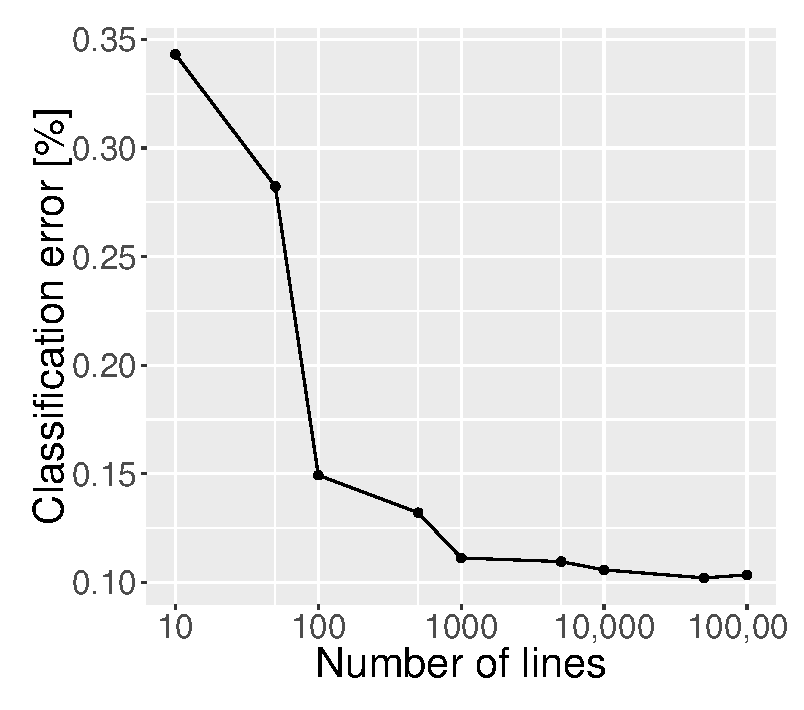
\includegraphics[height=7cm]{rf_error.eps}
	\caption{\label{rf_error} Validation error rate for subsets of different sizes.}
\end{figure}


The time to build the forest (i.e. excluding data loading and validation prediction) is shown in Figure~\ref{rf}a. Time increases roughly linearly with sample size. This is slightly unexpected, as R's vectorised operations should scale better than linearly with increased $n$.

Finally, as shown in shown in Figure~\ref{rf}b, the \texttt{randomForest} package uses a lot more RAM than what is required for the dataset, although usage scales linearly with $n$ as expected. The largest dataset \texttt{randomForest} was able to handle (100,000 lines) was \SI{7}{\mega\byte} on disk and \SI{9.2}{\mega\byte} when loaded into RAM, but \texttt{randomForest} used \SI{2700}{\mega\byte} to compute the random forest. This limitation seems to lie with the package, as R happily works with datasets significantly larger than that.

\begin{figure}[ht]
    \begin{subfigure}[t]{0.49\textwidth}
        \centering
        \includegraphics[height=6cm]{rf_time.eps}
        \caption{Forest build time.}
    \end{subfigure}%
    \begin{subfigure}[t]{0.49\textwidth}
        \centering
        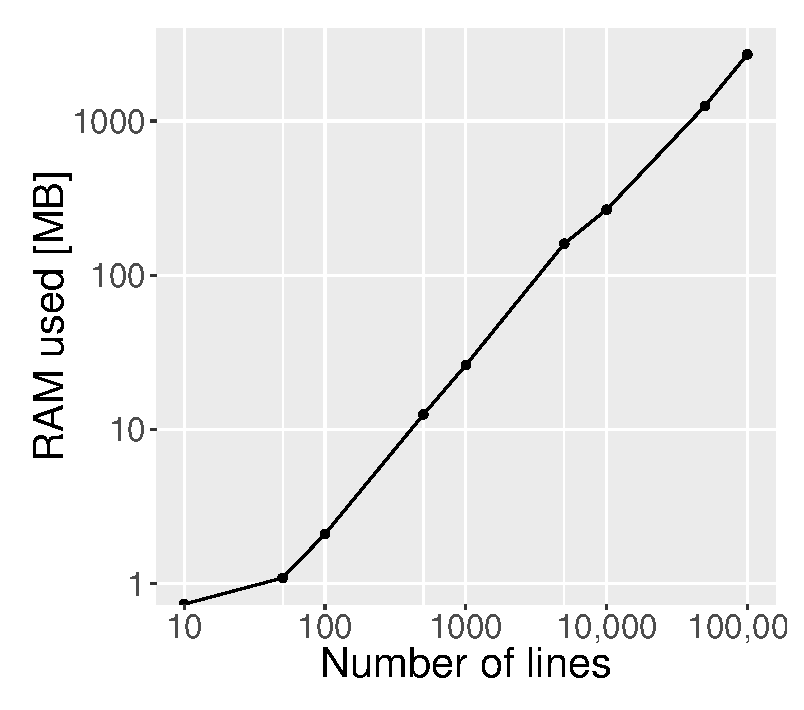
\includegraphics[height=6cm]{rf_ram.eps}
        \caption{Total RAM usage, including data and forest.}
    \end{subfigure}
    \caption{\label{rf} \texttt{randomForest} results for different subsets.}
\end{figure}

So while performance is acceptable for small datasets, \texttt{randomForest} is incapable of dealing with big-$n$ datasets in the 10s of MB.

\FloatBarrier



\subsection{\texttt{bigrf}}
\texttt{bigrf} is a package for creating classification random forests with large datasets. It uses the same basic algorithm as the standard \texttt{randomForest} package, with several advantages:

\begin{itemize}
    \item The algorithm is rewritten to reduce memory usage.
    \item The dataset, as well as each tree in the forest, are stored as type \texttt{big.matrix} from by the \texttt{bigmemory} package. \texttt{big.matrix}s are C++ objects, resulting in faster access speeds for many operations.
    \item \texttt{big.matrix} objets are stored in a part of RAM that is available to all processes, so running a computation on multiple cores means you only have one copy of the data in RAM, unlike the naive \texttt{mcapply} approach. 
    \item \texttt{big.matrix} objetcs can also be saved to disk instead of stored in memory. Although this is significantly slower than storing data in RAM, it allows for data larger than will fit in RAM. The different parts of the matrix are loaded into memory as required. The file is also available to all processes.
    \item Builtin support for parallel computation. This means forests can be created in multiple processes without replicating the data multiple times.
    \item No limit to the number of factor levels, so the destination airport feature can be included.
    \item Option to show useful statistics such as test errors and confusion matrix.
\end{itemize}

This extra performance comes at the expense of some drawbacks:
\begin{itemize}
    \item Only supported on Linux and OSX.
    \item More difficult to install.
    \item Can only be used for classification (not regression).
    \item The \texttt{big.matrix} cache files have to be manually deleted after each run.
\end{itemize}

The usage is similar to \texttt{randomForest}, and results in similar accuracies:

\begin{lstlisting}[frame=single, basicstyle=\footnotesize\ttfamily, language=R]
forest <- bigrfc(train.x, train.y, cachepath='/tmp/Rforest')
predictions <- predict(forest, valid.x, valid.y, cachepath='/tmp/Rpredict')
\end{lstlisting}
The cache paths for each operation refer to the location of the file to store the matrix in.

Figure~\ref{bigrf} shows the results of the \texttt{bigrf} classification. The classification error is approximately the same as for the \texttt{randomForest} package. The package was able to process the 2 million line dataset, but crashed on the 5 million line dataset. This is surprising, as the algorithm should handle files much larger than this.

\begin{figure}[ht]
    \begin{subfigure}[t]{0.49\textwidth}
        \centering
        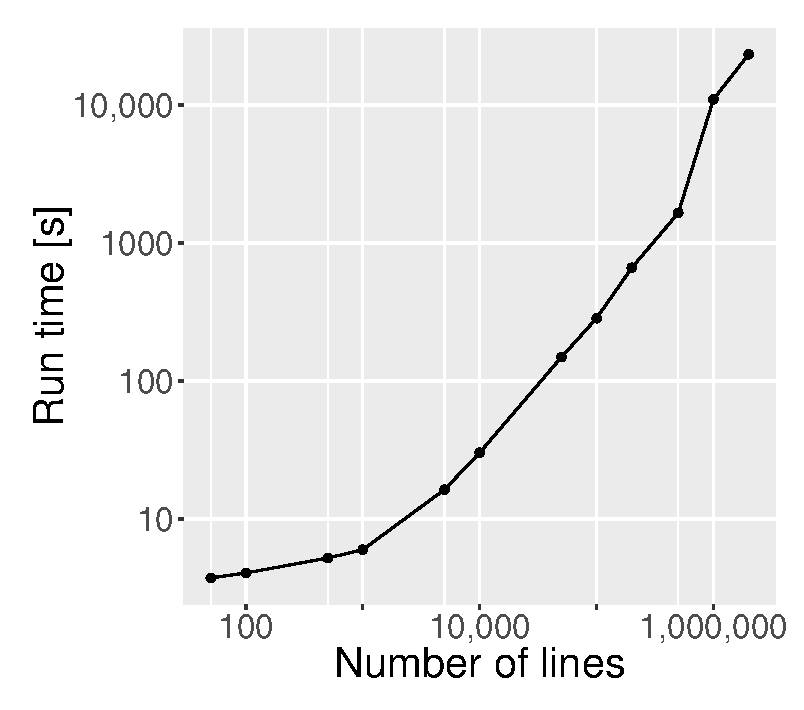
\includegraphics[height=6cm]{bigrf_time.eps}
        \caption{Forest build time.}
    \end{subfigure}%
    \begin{subfigure}[t]{0.49\textwidth}
        \centering
        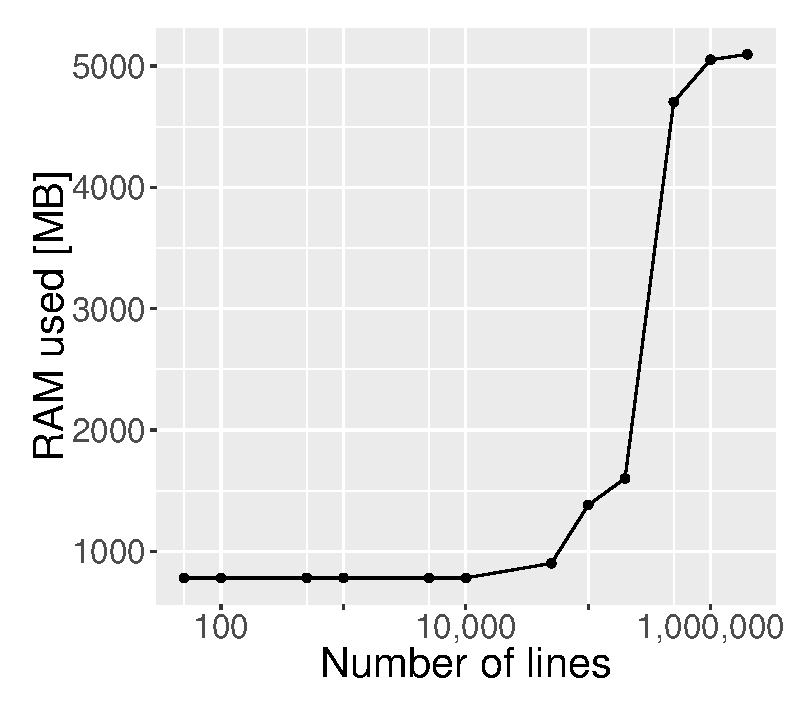
\includegraphics[height=6cm]{bigrf_ram.eps}
        \caption{Total RAM usage, including data and forest.}
    \end{subfigure}
    \caption{\label{bigrf} \texttt{randomForest} results for different size. \SI{10000}{\second} corresponds to roughly 2:45 hours.}
\end{figure}

\FloatBarrier

When creating new processes, each loads its own copy of the R environment, which takes up around \SI{150}{\mega\byte} per process. To prevent crashing, parallel computation had to be disabled at \SI{1000000}{lines} to free up more RAM.

The run time for the datasets increases roughly linearly until all the RAM is exhausted at around \SI{1000000}{lines}. Up until this point, it makes no difference whether disk caching is enabled for the  \texttt{big.matrix} objects. Once RAM is used up and the data starts to be read from disk, run time increases.

For small datasets, \texttt{bigrf} uses a significant amount of RAM. This is largely due to creating 4 new processes, each containing a copy of the R environment. The parallel computation setup also takes much more time than the actual forest creation for these small datasets also. As a result, it would be wise to disable parallel computation for very small datasets, or use the \texttt{randomForest} package.

For larger datasets, \texttt{bigrf} will use all the available RAM without crashing. It is surprising that the package crashed at all on the full dataset, though it is possible that some data is too big for RAM even when extracted from the disk-based matrix.

\section{Conclusion}
R is capable of working with large files and data frames, though care must be taken to chose the right tools. 

Although difficult to install, the \texttt{bigrf} package was just as easy to use as \texttt{randomForest}. In fact, \texttt{bigrf} has several usability advantages, including unlimited factor levels and builtin parallel computation.

\texttt{bigrf} is stable enough to handle much large datasets than \texttt{randomForest}. However, for small datasets the former uses much more RAM and takes much longer.


% \subsection{Chunking}
\clearpage
\bibliographystyle{plain}
\bibliography{references}
\end{document}
